%!TEX root = ./main.tex
\section{WCET estimation using model-checking}
\label{sec:modelchecking}

  WCET estimation can be reduced to a reachability problem in a network of timed
  automata~\cite{CB13}. The \textsc{Uppaal} tool that supports timed automata
  extended with bounded integer variables is used to build the models, and to
  solve the reachability problem.

  A model of the hardware is built where each architectural feature
  (pipeline(s), cache(s), bus(es), memory, \dots) is modeled by one or more
  timed automata. These automata are synchronized through {\it channels} to
  model the actual hardware behavior. For instance the automaton modeling the
  fetch stage of a pipeline is synchronized with the automaton modeling the
  instruction cache which is synchronized with the automaton modeling the bus
  and so on. The timings of the hardware are modeled by guards and clocks on
  some edges of the automata. A simple model of a memory controller could be the
  timed automaton of Figure~\ref{fig:memaccess}. Notice that this model accounts
  only for the timing.

  \begin{figure}[b]
    \raggedleft
    \floatbox[{\capbeside\thisfloatsetup{capbesideposition={right,center},capbesidewidth=9.3cm}}]{figure}[\FBwidth]
    {\caption{Simple modeling of a memory using \textsc{Uppaal}. In
        the initial state (on the top left) the memory waits for an
        access (MainMemStart synchronization channel). When the access
        is requested, clock $t$ resets and the automaton remains in
        the bottom right state until $t$ reaches the {\scriptsize
          MAINMEMTRANS} value. Then the memory returns to the initial
        state and notifies the end of the memory access (MainMemEnd
        synchronization channel).}\label{fig:memaccess}}
    {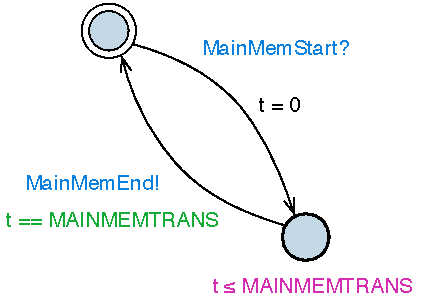
\includegraphics[scale=.6]{fig/automainmem.pdf}}
  \end{figure}

  A model of the program is automatically built from the binary code. In this
  model, each location corresponds to an instruction. An edge leaving a location
  corresponds to the execution of the instruction. For conditional branches, two
  edges leave the location according to the behavior of the branch (taken or not
  taken). Each edge is synchronized with the automaton that models the
  instruction fetch so that it may only be fired if the hardware fetches a new
  instruction. Memory locations are updated according to the semantics of the
  instruction and to its advance in the pipeline. The model of the program has
  an initial state, $I$, that corresponds to the entry point of the program and
  a final state, $F$, that corresponds to the point at which the WCET has to be
  computed.

  At last, a global clock $x$ is used to measure the time. It is initialized at
  0.

  The WCET is then the largest value, $max(x)$, of $x$ when $F$ is
  reached. $max(x)$ can be computed with a model-checker and the following
  reachability property $R(T)$: ``Is $F$ reachable with $x \geq T$ ?''. If
  $R(T)$ is true and $R(T+1)$ is false then $T$ is the WCET of the program.

  This approach is modular since the hardware and software models are built
  separately and the hardware model does not depend on the software to check. No
  assumption is made about the structure of the binary code generated by the
  compiler and the model of the program is built automatically without need for
  annotations

  \paragraph*{Modeling the values stored in memory}

  Data stored in memory and registers -- called a {\it location} in the
  remaining of the paper -- and used by the program can be either included in or
  abstracted away from the model.  Each location included in the model is
  associated with a bounded variable.  When the program accesses a location, the
  timing is computed by the models of the hardware.  If the location is included
  in the model, the associated variable is also read / written.  If the location
  is abstracted away, the data to be written is discarded and any read access
  returns the special value $\bot$.

  On the one hand, every location included in the model adds a dimension to the
  state of the system and thus contributes to the growth of the state space.  On
  the other hand, $\bot$ values can lead the model checker to explore paths that
  are not in the systems when they impact a conditional branch instruction.
  Thus the problem is to automatically compute the minimal set of locations that
  impact on the control flow of the program and that should be included in the
  model.  In this paper, we focus on this problem.

